% Concise flowchart of the formulation-4 RL (full version: flowchart.tex).
% Code: 2026-11-22_formulation_4/baseline_RL/code (train_rl_f4.py, rl_f4_model.rollout, rl_f4_env.Env, solve_rl_f4.py)
\documentclass[border=5pt]{standalone}
\usepackage{lmodern}
\usepackage[T1]{fontenc}
\usepackage{amsmath,amssymb}
\usepackage{tikz}
\usetikzlibrary{arrows.meta,shapes.geometric,shapes.misc,fit,backgrounds,calc}
\begin{document}
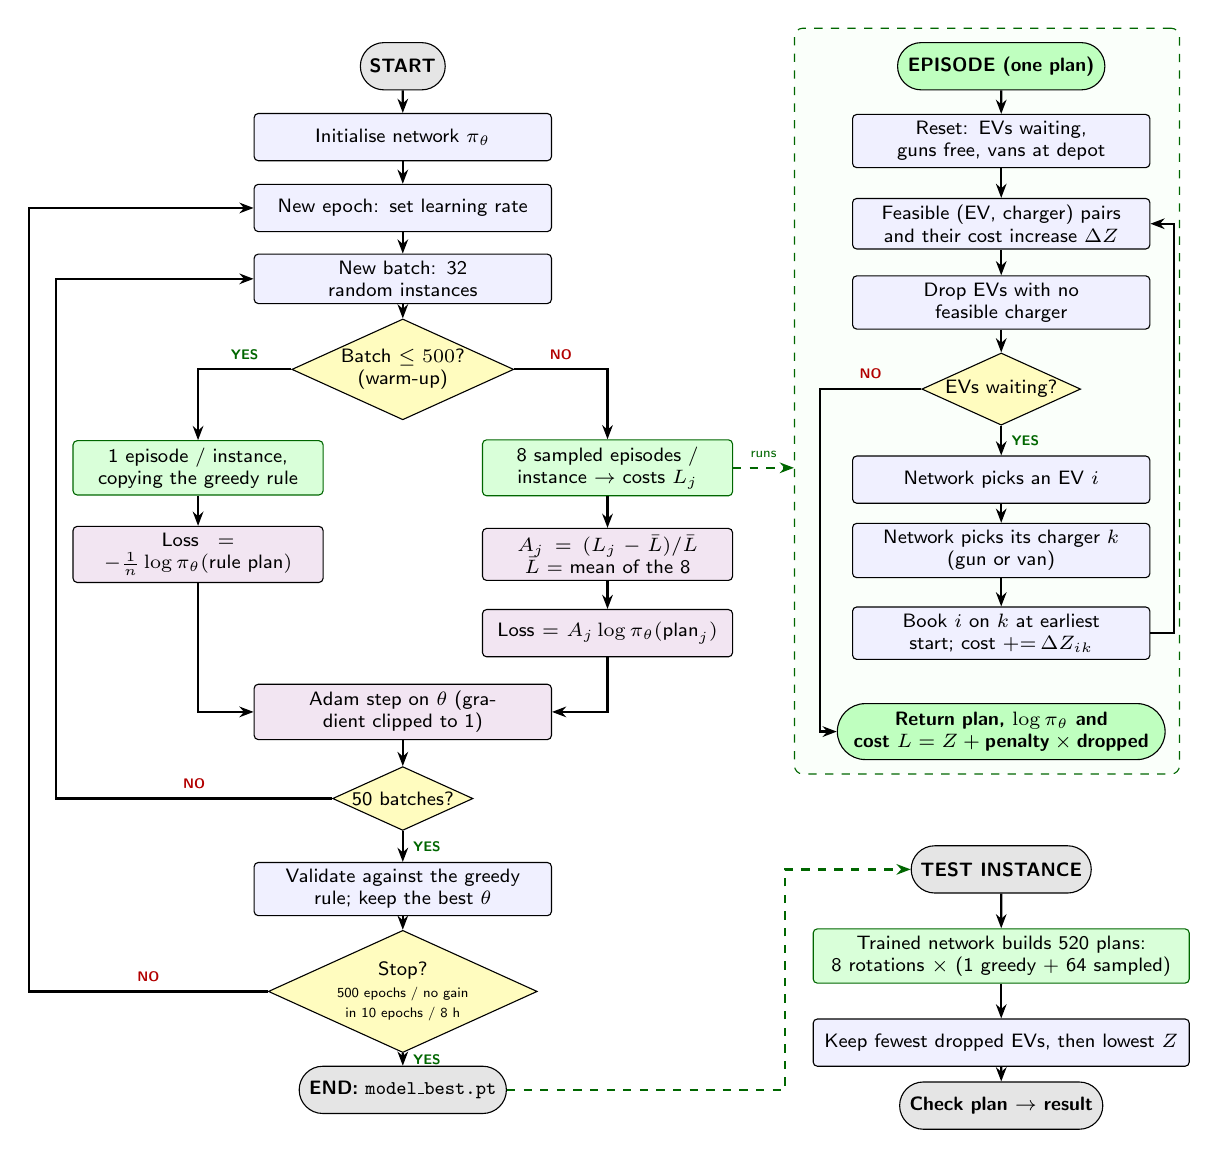
\begin{tikzpicture}[
  font=\sffamily\scriptsize, >={Stealth[length=1.8mm]},
  term/.style={rounded rectangle, draw, fill=gray!20, align=center, inner sep=3pt, minimum height=6mm, font=\sffamily\scriptsize\bfseries},
  box/.style={rectangle, rounded corners=1.5pt, draw, fill=blue!6, align=center, text width=#1, inner sep=2.5pt, minimum height=6mm},
  box/.default=3.6cm,
  lrn/.style={box=#1, fill=violet!10},
  lrn/.default=3.0cm,
  run/.style={box=#1, fill=green!15, draw=green!40!black},
  run/.default=3.0cm,
  dec/.style={diamond, draw, fill=yellow!25, aspect=2.2, align=center, inner sep=0.5pt},
  arr/.style={->, thick},
  yl/.style={font=\sffamily\tiny\bfseries, text=green!40!black},
  nl/.style={font=\sffamily\tiny\bfseries, text=red!70!black},
]
% ============================ TRAINING
\node[term] (s) at (0,0) {START};
\node[box] (init) at (0,-0.9) {Initialise network $\pi_\theta$};
\node[box] (ep) at (0,-1.8) {New epoch: set learning rate};
\node[box] (gen) at (0,-2.7) {New batch: 32 random instances};
\node[dec] (w) at (0,-3.85) {Batch $\le 500$?\\(warm-up)};
\node[run] (w1) at (-2.6,-5.1) {1 episode / instance,\\ copying the greedy rule};
\node[lrn] (w2) at (-2.6,-6.2) {$\text{Loss}=-\tfrac1n\log\pi_\theta(\text{rule plan})$};
\node[run] (r1) at (2.6,-5.1) {8 sampled episodes / instance $\to$ costs $L_j$};
\node[lrn] (r2) at (2.6,-6.2) {$A_j=(L_j-\bar L)/\bar L$\\ $\bar L$ = mean of the 8};
\node[lrn] (r3) at (2.6,-7.2) {$\text{Loss}=A_j\log\pi_\theta(\text{plan}_j)$};
\node[lrn=3.6cm] (adam) at (0,-8.2) {Adam step on $\theta$ (gradient clipped to 1)};
\node[dec] (b) at (0,-9.3) {50 batches?};
\node[box] (val) at (0,-10.45) {Validate against the greedy rule; keep the best $\theta$};
\node[dec] (st) at (0,-11.75) {Stop?\\ \tiny 500 epochs / no gain\\[-1pt] \tiny in 10 epochs / 8 h};
\node[term] (e) at (0,-13.0) {END: \texttt{model\_best.pt}};
\draw[arr] (s)--(init); \draw[arr] (init)--(ep); \draw[arr] (ep)--(gen); \draw[arr] (gen)--(w);
\draw[arr] (w.west) -| node[yl, above, pos=0.25]{YES} (w1);
\draw[arr] (w.east) -| node[nl, above, pos=0.25]{NO} (r1);
\draw[arr] (w1)--(w2); \draw[arr] (r1)--(r2); \draw[arr] (r2)--(r3);
\draw[arr] (w2) |- (adam.west); \draw[arr] (r3) |- (adam.east);
\draw[arr] (adam)--(b);
\draw[arr] (b.west) -- node[nl, above]{NO} (-4.4,-9.3) |- (gen.west);
\draw[arr] (b) -- node[yl, right]{YES} (val);
\draw[arr] (val)--(st);
\draw[arr] (st.west) -- node[nl, above]{NO} (-4.75,-11.75) |- (ep.west);
\draw[arr] (st) -- node[yl, right]{YES} (e);

% ============================ ONE EPISODE
\begin{scope}[xshift=7.6cm]
\node[term, fill=green!25] (a0) at (0,0) {EPISODE (one plan)};
\node[box] (a1) at (0,-0.95) {Reset: EVs waiting, guns free, vans at depot};
\node[box] (a2) at (0,-2.0) {Feasible (EV, charger) pairs and their cost increase $\Delta Z$};
\node[box] (a3) at (0,-3.0) {Drop EVs with no feasible charger};
\node[dec] (a4) at (0,-4.1) {EVs waiting?};
\node[box] (a5) at (0,-5.25) {Network picks an EV $i$};
\node[box] (a6) at (0,-6.15) {Network picks its charger $k$\\ (gun or van)};
\node[box] (a7) at (0,-7.2) {Book $i$ on $k$ at earliest start; cost $+{=}\,\Delta Z_{ik}$};
\node[term, fill=green!25] (a8) at (0,-8.45) {Return plan, $\log\pi_\theta$ and\\ cost $L=Z+\text{penalty}\times\text{dropped}$};
\draw[arr] (a0)--(a1); \draw[arr] (a1)--(a2); \draw[arr] (a2)--(a3); \draw[arr] (a3)--(a4);
\draw[arr] (a4) -- node[yl, right]{YES} (a5); \draw[arr] (a5)--(a6); \draw[arr] (a6)--(a7);
\draw[arr] (a7.east) -- ++(0.3,0) |- (a2.east);
\draw[arr] (a4.west) -- node[nl, above]{NO} (-2.3,-4.1) |- (a8.west);
\coordinate (pad) at (-2.45,-4.1);
\end{scope}
\begin{scope}[on background layer]
  \node[draw=green!40!black, dashed, rounded corners=3pt, fill=green!2, fit=(a0)(a1)(a7)(a8)(pad), inner sep=5pt] (fr) {};
\end{scope}
\draw[->, dashed, thick, green!40!black] (r1.east) -- node[above, font=\sffamily\tiny]{runs} (fr.west|-r1.east);

% ============================ AFTER TRAINING
\begin{scope}[xshift=7.6cm, yshift=-10.2cm]
\node[term] (i0) at (0,0) {TEST INSTANCE};
\node[run=4.6cm] (i1) at (0,-1.1) {Trained network builds 520 plans:\\ 8 rotations $\times$ (1 greedy + 64 sampled)};
\node[box=4.6cm] (i2) at (0,-2.2) {Keep fewest dropped EVs, then lowest $Z$};
\node[term] (i3) at (0,-3.0) {Check plan $\to$ result};
\draw[arr] (i0)--(i1); \draw[arr] (i1)--(i2); \draw[arr] (i2)--(i3);
\end{scope}
\draw[->, dashed, thick, green!40!black] (e.east) -| ($(i1.west|-i0.west)+(-0.35,0)$) -- (i0.west);
\end{tikzpicture}
\end{document}
